\documentclass{beamer}
\usepackage{graphicx}
\usepackage{xcolor}
\usepackage{ctex}
\usepackage{amsmath}
\usepackage{amssymb}
\usepackage{xeCJK}
\hypersetup{colorlinks,linkcolor = green, urlcolor = green}

\title{非抢占式内核}
\subtitle{任务 1:多 tasks 启动与 context switch}
\institute{University of Chinese Academy of Sciences}
\author{冯吕,张旭}
\date{\today}
\usetheme{Hannover}
\begin{document}

\begin{frame}
\titlepage
\begin{figure}[ht]\centering
\includegraphics[scale=0.3]{ucas.jpg}\end{figure}
\end{frame}

\begin{frame}{Outline}
\tableofcontents
\end{frame}
 
\section{任务}
\begin{frame}{概述}
整个task的实现。
\begin{figure}
	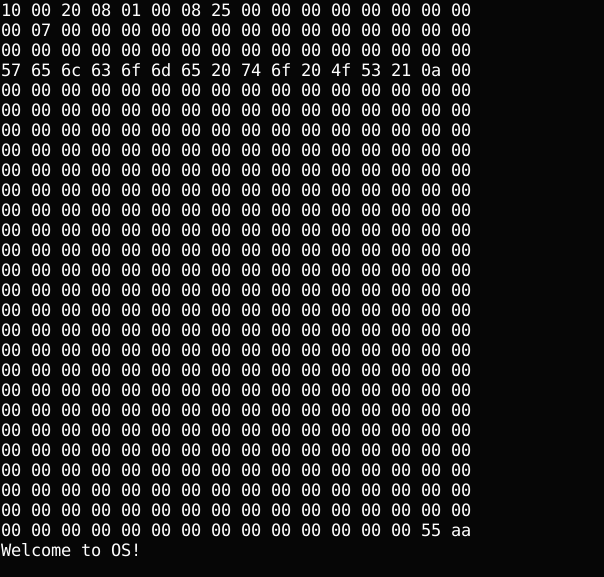
\includegraphics[scale=0.12]{2.png}
\end{figure}
\end{frame}
\begin{frame}
\frametitle{函数以及函数调用关系}
\begin{itemize}
	\item $bootblock\text{读盘}\Rightarrow \_stat()$\\
	$\_stat()$函数完成$PCB$的初始化和准备队列的初始化,之后调用$scheduler\_entry()$启动进程(线程$1$);\\
	
	\item $scheduler\_entrry()\Rightarrow scheduler()\Rightarrow$启动第一个进程\\
	\item 线程切换:$do\_yield()\Rightarrow save\_PCB() \&\& queue\_push 
	scheduler\_entry()$\\
	\item 进程切换:$yield()\Rightarrow \text{系统调用}\Rightarrow do\_yield()$
\end{itemize}
\end{frame}

\begin{frame}{任务}
需要实现下面的函数:
\begin{itemize}
	\item 修改createimage,需要将process1,2,3也写入image.
	\item $PCB$的设置
	\item 栈的设置
	\item $\_stat()$:初始化$PCB$和准备队列。
	\item $save\_pcb()$:保存上下文
	\item $scheduler\_entry()$:选取下一个进程来运行
	\item ...
\end{itemize}
\end{frame}


\section{实现}
\begin{frame}{PCB 结构}
需要保存的信息:
\begin{itemize}
	\item $s0\sim s7$:寄存器变量,切换时需要保存。
	\item $sp$:栈指针
	\item $ra$:返回地址
	\item 进程状态(在任务一中暂时没什么用)。
\end{itemize}
\end{frame}

\begin{frame}{栈的设置}
不能过大,否则$\Rightarrow$ TLB miss.

不能太小,否则与进程地址冲突。 
\end{frame}

\begin{frame}{函数实现}
看代码。
\end{frame}

\section{问题及解决方法}
\begin{frame}{入口地址变化}
\begin{itemize}
	\item 在实验一中,读完盘后调到 \emph{0xa080026c} 处执行。\\
	\item 在实验二中,$\_stat()$函数的入口地址变为\emph{0xa08002bc}.
	
\end{itemize}
\end{frame}

\begin{frame}{PCB信息存储}
\begin{itemize}
	\item 队列结构中只有一个 PCB 指针的指针,kernel.c 
	中有一个PCB指针数组,所以还需要自己声明一个PCB数组存储信息。
	\item $queue->pcbs \Rightarrow ready\_array[]\Rightarrow$真正存储PCB信息的数组
\end{itemize}
\end{frame}

\begin{frame}{栈的设置}
\begin{itemize}
	\item 栈的设置过大,导致跳到线程1压栈时出现TLB miss.
	\item 减小栈的地址。
	\item 貌似一开始没有什么好的方法来确定,只能通过出错来摸索。
\end{itemize}
\end{frame}

\begin{frame}{保存 PCB 出错}
保存 PCB 的时候sp 和ra 会发生变化。
\begin{figure}
	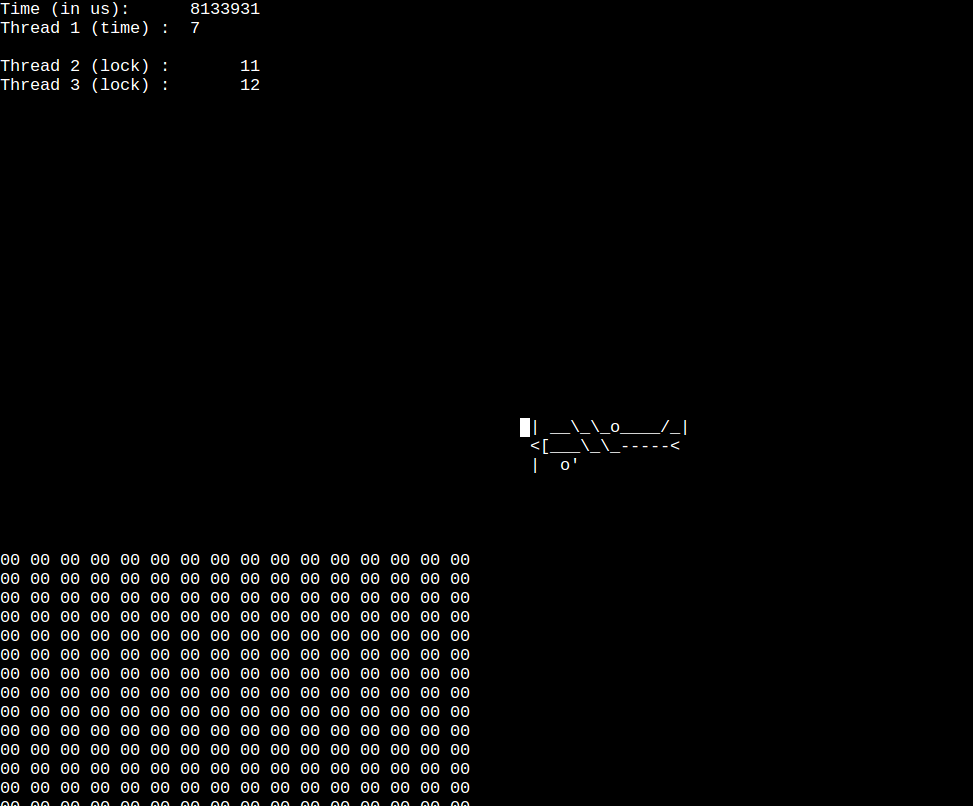
\includegraphics[scale=0.5]{1.png}
\end{figure}
\end{frame}

\begin{frame}{kernel 入口地址}
\begin{itemize}
	\item 刚开始忘记修改kernel入口地址,导致进入process1后无法切换到
	内核态。
\end{itemize}
\end{frame}

\end{document}
